\documentclass[aspectratio=169,11pt]{beamer}

\usepackage[utf8]{inputenc}
\usepackage[T1]{fontenc}
\usepackage[brazil]{babel}
\usepackage{amsmath,amssymb}
\usepackage{graphicx}
\usepackage{tikz}
\usepackage{booktabs}
\usepackage{xcolor}
\usepackage{array}
\usepackage{multicol}
\usepackage{algorithm}
\usepackage{algpseudocode}
\usepackage{lmodern}

\makeatletter
\renewcommand{\alglinenumber}[1]{\tiny #1}
\makeatother

% Definição do comando argmax e argmin
\DeclareMathOperator*{\argmax}{arg\,max}
\DeclareMathOperator*{\argmin}{arg\,min}

\usetikzlibrary{positioning,shapes.geometric,arrows.meta,shadows,calc}

\usetheme{Madrid}
\usecolortheme{seahorse}

\setbeamertemplate{navigation symbols}{}
\setbeamertemplate{itemize items}[circle]
\setbeamercolor{itemize item}{fg=blue!70!black}
\setbeamercolor{enumerate item}{fg=blue!70!black}

% Rodapé personalizado com meu nome
\setbeamertemplate{footline}{%
  \leavevmode%
  \hbox{%
    \begin{beamercolorbox}[wd=0.22\paperwidth,ht=2.5ex,dp=1ex,left]{author in head/foot}%
      \hspace{0.2cm}%
      \textbf{Luryan Delevati Dorneles}
    \end{beamercolorbox}%
    \begin{beamercolorbox}[wd=0.63\paperwidth,ht=2.5ex,dp=1ex,center]{title in head/foot}%
      \usebeamerfont{title in head/foot}\insertshorttitle%
    \end{beamercolorbox}%
    \begin{beamercolorbox}[wd=0.15\paperwidth,ht=2.5ex,dp=1ex,right]{date in head/foot}%
      \insertframenumber{} / \inserttotalframenumber\hspace{0.2cm}%
    \end{beamercolorbox}%
  }%
  \vskip0pt%
}

% Cores personalizadas
\definecolor{ufal}{RGB}{0,85,150}
\definecolor{accent}{RGB}{200,100,50}
\definecolor{success}{RGB}{46,125,50}

% Configurações de fonte
\setbeamerfont{title}{size=\Large,series=\bfseries}
\setbeamerfont{subtitle}{size=\normalsize}
\setbeamerfont{frametitle}{size=\large,series=\bfseries}

% Logo no header - sem quebra de content
\addtobeamertemplate{frametitle}{}{%
  \begin{tikzpicture}[remember picture,overlay]
    \node[anchor=north east] at ($(current page.north east) + (-0.5cm,0.2cm)$) 
      {\includegraphics[height=1.4cm]{img/ufal1.png}};
  \end{tikzpicture}%
}

\title[Otimização da Observação Ambiental em UCs]{Otimização da Observação Ambiental em Unidades de Conservação:\\Integração de Heurística e Programação Linear Inteira Mista}

\author[Dorneles et al.]{L. D. Dorneles \and Í. B. Q. Araujo \and G. R. Leite \and R. G. S. Pinheiro \and B. C. S. Nogueira}

\institute[UFAL]{Universidade Federal de Alagoas}
\date{SBPO 2025}

\begin{document}

% Slide 1: Título com logos ajustados
\begin{frame}[plain]
    \begin{tikzpicture}[remember picture,overlay]
        % Main content
        \node[text width=12cm,align=center] at (current page.center) {
            {\fontsize{17}{21}\selectfont\textbf{\color{ufal}Otimização da Observação Ambiental em Unidades de Conservação}}\\[0.3cm]
            {\fontsize{14}{16}\selectfont\color{black!80}Integração de Heurística e Programação Linear Inteira Mista}\\[0.8cm]
            
            {\footnotesize\textbf{Luryan D. Dorneles, Ícaro B. Q. Araujo, Glauber R. Leite,\\
            Rian G. S. Pinheiro, Bruno C. S. Nogueira}}\\[0.5cm]
            
            % Logo do IC e SBPO lado a lado, centralizados
            \includegraphics[height=1.3cm]{img/ufal.jpg}\hspace{0.5cm}%
            \includegraphics[height=1.3cm]{img/logo-ic.png}\hspace{0.8cm}%
            \includegraphics[height=1.3cm]{img/sbpo2025-header-logo.png}\\[0.2cm]
            
            {\scriptsize Universidade Federal de Alagoas \quad|\quad SBPO 2025}
        };
    \end{tikzpicture}
\end{frame}

% Slide 2: Introdução
\begin{frame}{Observação Ambiental com Imagens de Satélite}
\vspace{-0.3cm}
\begin{columns}[T]
    \begin{column}{0.6\textwidth}
        \textbf{\color{ufal}Desafio Principal:}
        \begin{itemize}
            \item Como observar \textbf{eficientemente} UCs ao longo do tempo?
            \item Milhares de imagens disponíveis
            \item Qualidade variável (nuvens, dados faltantes)
        \end{itemize}
        
        \vspace{0.4cm}
        \textbf{\color{success}Abordagem Proposta:}
        \begin{itemize}
            \item Método \textbf{híbrido} (Heurística Gulosa + PLIM)
            \item Seleção automática e ótima
            \item Métricas de qualidade
            \item Cobertura temporal consistente
        \end{itemize}
    \end{column}
    \begin{column}{0.35\textwidth}
        \begin{tikzpicture}
            \node[draw,circle,minimum size=2cm,fill=ufal!20,text width=1.8cm,align=center,font=\scriptsize] 
                (inicio) {1.941\\Imagens\\Candidatas};
            \draw[->,thick,ufal] (inicio) -- (0,-1.8);
            \node[draw,circle,minimum size=1.6cm,fill=orange!20,text width=1.4cm,align=center,font=\scriptsize] 
                (heuristica) at (0,-2.4) {524\\Imagens\\Filtradas};
            \draw[->,thick,orange] (heuristica) -- (0,-3.6);
            \node[draw,circle,minimum size=1.4cm,fill=success!20,text width=1.2cm,align=center,font=\scriptsize] 
                (final) at (0,-4.2) {~74\\Imagens\\Utilizadas};
        \end{tikzpicture}
    \end{column}
\end{columns}
\end{frame}

% Slide 3: Conceito de mosaicos
\begin{frame}{Mosaicos de Imagens de Satélite}
\vspace{-0.6cm}
\begin{center}
    \colorbox{ufal!10}{\parbox{0.8\textwidth}{\centering\textbf{\color{ufal}MOSAICO = Conjunto de imagens que cobrem uma área}}}
\end{center}

\vspace{0.2cm}
\begin{columns}[T,onlytextwidth]
    \begin{column}{0.55\textwidth}
        \includegraphics[width=\textwidth,height=4.0cm,keepaspectratio]{img/mosaic_example.jpg}
    \end{column}
    \begin{column}{0.45\textwidth}
        \begin{itemize}
            \item Cada imagem cobre \textbf{parte} da região
            \vspace{0.2cm}
            \item Com sobreposição, criam o \textbf{efeito} de uma única imagem
            \vspace{0.2cm}
            \item \textbf{\color{accent}Qual a melhor combinação escolher?}
        \end{itemize}
        
        \vspace{0.4cm}
        \begin{center}
            \tikz{\node[draw,rounded corners,fill=success!15,text width=5.0cm,align=center,font=\footnotesize] 
                {\textbf{Problema NP-difícil:} (Kumar \& Ramesh, 1995; Masek, 1978)};}
        \end{center}
    \end{column}
\end{columns}
\end{frame}

% Slide 4: Desafios mais organizados
\begin{frame}{Desafios do Monitoramento}
\vspace{-0.2cm}
\begin{multicols}{3}
    \begin{center}
        \tikz{\node[draw,circle,fill=red!20,minimum size=1.2cm,font=\tiny]{NUVENS};}\\
        \textbf{Problema 1}\\
        {\footnotesize Até 40\% da imagem inútil}
    \end{center}
    
    \columnbreak%
    \begin{center}
        \tikz{\node[draw,circle,fill=orange!20,minimum size=1.2cm,font=\tiny]{PIXELS};}\\
        \textbf{Problema 2}\\
        {\footnotesize Dados faltantes/inválidos}
    \end{center}
    
    \columnbreak%
    \begin{center}
        \tikz{\node[draw,circle,fill=blue!20,minimum size=1.2cm,font=\tiny]{TEMPO};}\\
        \textbf{Problema 3}\\
        {\footnotesize Análise multitemporal}
    \end{center}
\end{multicols}

\vspace{0.3cm}
\begin{center}
    \colorbox{accent!10}{\parbox{8cm}{\centering\textbf{Necessário:} Selecionar a mesma área em diferentes períodos}}
\end{center}
\end{frame}

% Slide 5: Visualização dos problemas na prática
\begin{frame}{Problemas Visuais: Nuvens e Cobertura}
\vspace{-0.5cm}
\begin{center}
    \includegraphics[width=0.45\textwidth]{img/visualizacao_clouds_and_outfovcorner.jpg}
\end{center}
\vspace{-0.2cm}
\begin{center}
    \footnotesize\textbf{Exemplo real:} Nuvens (branco) e dados faltantes prejudicam o monitoramento
\end{center}
\end{frame}

% Slide 19: Comparação com Literatura
\begin{frame}{Contexto e Perspectiva Científica}
\vspace{-0.2cm}
\begin{center}
\textbf{Visão da otimização multidimensional:}
\end{center}

\begin{columns}[T]
    \begin{column}{0.48\textwidth}
        \textbf{\color{ufal}Trabalhos relacionados:}
        \begin{itemize}
            \item Rodriguez-Puerta et al\@.: Apenas remoção de nuvens (89,4\%)
            \item Shepherd et al\@.: Qualidade radiométrica sazonal (<0,1\% nuvens)
            \item Combarro-Simon: Heurística gulosa simples
        \end{itemize}
    \end{column}
    \begin{column}{0.48\textwidth}
        \textbf{\color{success}Contribuições desta Pesquisa:}
        \begin{itemize}
            \item Otimização multidimensional
            \item Sequências temporais consistentes
            \item Heurística + PLIM híbrida
            \item Exclusividade de imagens
        \end{itemize}
    \end{column}
\end{columns}
\end{frame}

% Slide 6: Áreas de estudo
\begin{frame}{Unidades de Conservação Estudadas}
\vspace{-0.6cm}
\begin{center}
    \textbf{\large 13 UCs em 9 Estados Brasileiros}
\end{center}

\vspace{-0.6cm}
\begin{columns}[c]
    \begin{column}{0.35\textwidth}
        \includegraphics[width=\textwidth,height=3.5cm,keepaspectratio]{img/mosaic_top1_output-each-area.jpg}
    \end{column}
    \begin{column}{0.63\textwidth}
        \begin{multicols}{2}
        {\scriptsize
        \textbf{MG---SP---RJ:}\\
        • PARNA Mantiqueira\\
        \quad (437.192 ha)\\[3pt]
        
        \textbf{Rio Grande do Sul:}\\
        • APA Ibirapuitã\\
        \quad (318.767 ha)\\[3pt]
        
        \textbf{Mato Grosso:}\\
        • PARNA Pantanal\\
        \quad (33.800 ha)\\[3pt]
        
        \textbf{Alagoas:}\\
        • APA Muricy (129.742 ha)\\
        • APA Santa Rita (9.633 ha)\\
        • APA Catolé (3.708 ha)\\
        • APA Pratagy (20.873 ha)\\[3pt]
        
        \columnbreak%
        
        \textbf{Bahia:}\\
        • PARNA Pau Brasil\\
        \quad (18.934 ha)\\
        • PARNA Monte Pascoal\\
        \quad (22.239 ha)\\
        • PARNA Descobrimento\\
        \quad (22.607 ha)\\
        • REVIS Rio dos Frades\\
        \quad (907 ha)\\[3pt]
        
        \textbf{PI---PE---CE:}\\
        • APA Chapada Araripe\\
        \quad (1.019.460 ha)\\
        • FLONA Araripe-Apodi\\
        \quad (38.920 ha)
        }
        \end{multicols}
    \end{column}
\end{columns}
\end{frame}

% Slide 7: Metodologia
\begin{frame}{Metodologia Híbrida}
\vspace{-0.2cm}
\begin{center}
\begin{columns}[c]
    \begin{column}{0.25\textwidth}
        \begin{center}
            \colorbox{blue!20}{\parbox{2.5cm}{\centering\footnotesize\textbf{FASE 1}\\Heurística\\Gulosa}}\\[0.2cm]
            
            \textcolor{blue}{\Large$\downarrow$}\\[0.2cm]
            
            \colorbox{green!20}{\parbox{2.5cm}{\centering\footnotesize Mosaicos\\Candidatos}}\\[0.2cm]
            
            \textcolor{green}{\Large$\downarrow$}\\[0.2cm]
            
            \colorbox{orange!20}{\parbox{2.5cm}{\centering\footnotesize\textbf{FASE 2}\\Modelo\\PLIM}}\\[0.2cm]
            
            \textcolor{orange}{\Large$\downarrow$}\\[0.2cm]
            
            \colorbox{success!30}{\parbox{2.5cm}{\centering\footnotesize Mosaicos\\Ótimos}}
        \end{center}
    \end{column}
    
    \begin{column}{0.7\textwidth}
        \textbf{Fase 1 --- Heurística Gulosa:}
        \begin{itemize}
            \item Calcula efetividade das imagens
            \item Forma grupos compatíveis
            \item Cobertura mínima de 85\%
        \end{itemize}
        
        \vspace{0.3cm}
        \textbf{Fase 2 --- Otimização:}
        \begin{itemize}
            \item Modelo PLIM para seleção final
            \item Maximiza cobertura útil
            \item Minimiza nuvens
            \item Garante sobreposição $\geq$ 80\%
        \end{itemize}
    \end{column}
\end{columns}
\end{center}
\end{frame}

% Slide 8: Tabela de Notação
\begin{frame}{Notação}
\vspace{-0.2cm}
\begin{columns}[T]
    \begin{column}{0.48\textwidth}
        \begin{itemize}
            \item $I$ = Imagens Sentinel-2 candidatas
            \item $A$ = Área de Interesse (UC)
            \item $A_i$ = Cobertura geográfica da imagem $i$
            \item $P_i$ = Proporção de pixels válidos
            \item $N_i$ = Proporção de nuvens
            \item $\Delta T_{\max}$ = Janela temporal (5 dias)
        \end{itemize}
    \end{column}
    \begin{column}{0.48\textwidth}
        \begin{itemize}
            \item $E_i$ = Efetividade da imagem $i$
            \item $M_{novo}$ = Mosaico em construção
            \item $I_{comp}$ = Imagens compatíveis temporais
            \item $\Delta A^{\min}$ = Incremento mínimo (5\%)
            \item $A_M^{\text{alvo}}$ = Cobertura alvo (85\%)
            \item $Q_i$ = Fator de qualidade da imagem $i$
        \end{itemize}
    \end{column}
\end{columns}
\end{frame}

% Slide 9: Pseudocódigo
\begin{frame}{Algoritmo de Seleção de Mosaicos}
\vspace{-0.3cm}

\begin{algorithm}[H]
\tiny
\caption{Seleção de mosaicos candidatos}
\begin{algorithmic}[1]
\State%
\textbf{Entrada:} $I$, $A$, $\Delta T_{\max}$, $\Delta A^{\min}$, $A_M^{\text{alvo}}$, $A_M^{\min}$, $N_M^{\max}$
\State%
\textbf{Saída:} $M$
\State%
Inicializar $M \gets \emptyset$; filtrar $I$ com $N_i \leq N_M^{\max}$
\While{há regiões de $A$ não cobertas}
    \State%
    $M_{novo} \gets \emptyset$
    \State% 
    Para cada $i \in I$, calcular $E_i = A_i \cdot P_i \cdot Q_i$ (Efetividade)
    \State%
    Selecionar $i^* = \argmax_{i \in I} E_i$ como semente
    \State%
    Definir $I_{comp} = \{i \in I : |t_i - t_{i^*}| \leq \Delta T_{\max}\}$ (compatíveis temporais)
    \While{$I_{comp} \neq \emptyset$ e cobertura pode ser melhorada}
        \State%
        Para cada $i \in I_{comp}$, calcular $E_i$; definir $I'_{comp}$ com sobreposição válida
        \State% 
        Selecionar $i^* = \argmax_{i \in I'_{comp}} E_i$
        \If{$i^*$ aumenta cobertura em $\geq \Delta A^{\min}$}
            \State%
            Adicionar $i^*$ ao $M_{novo}$; atualizar $I_{comp}$ para janela temporal
        \Else%
            \State%
            $I_{comp} \gets \emptyset$ (parada: sem melhoria)
        \EndIf%
    \EndWhile%
    \If{Cobertura ($M_{novo}$) $\geq A_M^{\min}$ (85\%)}
        \State%
        Adicionar $M_{novo}$ a $M$
    \EndIf%
\EndWhile%
\State%
\textbf{Aplicar PLIM} nos mosaicos candidatos $M$ para seleção ótima
\State%
\textbf{Retornar} Mosaicos selecionados
\end{algorithmic}
\end{algorithm}
\end{frame}

% novo slide 10: resultados heuristica
\begin{frame}{Resultados da Heurística Gulosa}
\vspace{-0.3cm}
\begin{center}
\textbf{Mosaicos candidatos gerados por região:}
\end{center}

\begin{center}
\footnotesize
\begin{tabular}{llcccc}
\toprule
\textbf{UF} & \textbf{UC} & \textbf{Área (ha)} & \textbf{Imagens} & \textbf{Mosaicos} & \textbf{Nuvens} \\
 & & & \textbf{(aceitas)} & \textbf{H. Gulosa} & \textbf{máx. (\%)} \\
\midrule
MG-SP-RJ & PARNA Mantiqueira & 437.192 & 179 & 45 & 37,83 \\
RS & APA Ibirapuitã & 318.767 & 54 & 16 & 10,77 \\
MT & PARNA do Pantanal & 33.800 & 52 & 18 & 9,12 \\
AL & APAs (4 unidades) & 163.956 & 80 & 24 & 38,91 \\
BA & PARNAs + REVIS (4 unid.) & 64.687 & 37 & 9 & 38,68 \\
PI-PE-CE & APA + FLONA (2 unid.) & 1.058.380 & 106 & 46 & 26,77 \\
\midrule
\textbf{Total} & \textbf{13 UCs} & \textbf{2.076.762} & \textbf{524} & \textbf{158} & \textbf{---} \\
\bottomrule
\end{tabular}
\end{center}

\vspace{0.3cm}
\begin{itemize}
\item \textbf{Entrada:} 1.941 imagens → \textbf{Filtradas:} 508 imagens aceitas
\item \textbf{Gerados:} 158 mosaicos candidatos pela heurística
\item \textbf{Variação climática:} De 9,12\% (MT) até 38,91\% (AL) de nuvens
\end{itemize}
\end{frame}

% slide novo: variavel do modelo 
\begin{frame}{Variáveis do Modelo PLIM}
\vspace{-0.2cm}
    \begin{itemize}
        \item $y_j$ = Variável binária de seleção do mosaico $j$
        \item $E_j$ = Cobertura efetiva do mosaico $j$
        \item $N_j$ = Proporção de nuvens do mosaico $j$
        \item $\gamma$ = Peso de penalização por nuvens
        \item $N_{\max}$ = Número máximo de mosaicos
        \item $I_{j,k}$ = Sobreposição entre mosaicos $j$ e $k$
    \end{itemize}
\end{frame}

% Slide 11: Função objetivo
\begin{frame}{Modelo PLIM:\@ Função Objetivo e Restrições}
\vspace{-1.0cm}
\begin{center}
    \colorbox{ufal!10}{\parbox{8cm}{\centering
        \textbf{Maximizar:}\\[0.2cm]
        {\Large $\sum_j E_j \cdot y_j - \gamma \sum_j N_j \cdot y_j$}
    }}
\end{center}

\vspace{0.3cm}
\textbf{Componentes da função objetivo:}
\begin{itemize}
    \item \textbf{Termo 1:} Efetividade da cobertura útil ($E_j$)
    \item \textbf{Termo 2:} Penalização por nuvens ($\gamma \times N_j$)
\end{itemize}

\vspace{0.2cm}
\footnotesize\textbf{Resultado:} Prioriza mosaicos com alta cobertura e baixa nebulosidade
\end{frame}

% Slide 12: Detalhamento das Restrições do Modelo PLIM
\begin{frame}{Restrições do Modelo PLIM}
\vspace{-0.2cm}
\textbf{Restrições principais do modelo de otimização:}

\begin{enumerate}
    \item \textbf{Limite de mosaicos:} $\sum_{j \in M} y_j \leq N_{\max}$
    \begin{itemize}
        \item Evita fragmentação excessiva
        \item Facilita análise temporal
    \end{itemize}
    
    \item \textbf{Exclusividade de imagens:} $\sum_{j \in M(i)} y_j \leq 1 \quad \forall i \in I'$
    \begin{itemize}
        \item Cada imagem em no máximo 1 mosaico
        \item Elimina redundâncias
    \end{itemize}
    
    \item \textbf{Sobreposição mínima:} $y_j + y_k \leq 1 \quad \forall j,k \mid I_{j,k} < 80\%$
    \begin{itemize}
        \item Garante continuidade espacial
        \item Permite comparação multitemporal
    \end{itemize}
\end{enumerate}
\end{frame}

% Slide 14: Resultados Experimentais
\begin{frame}{Resultados Heurística vs PLIM}
\vspace{-0.2cm}
\begin{center}
\textbf{Redução significativa no número de mosaicos:}
\end{center}

\begin{center}
\begin{tabular}{lccc}
\toprule
\textbf{Região} & \textbf{Candidatos} & \textbf{Selecionados} & \textbf{Redução (\%)} \\
\midrule
MG-SP-RJ    & 45 & 6 & 86,7\% \\
RS          & 16 & 5 & 68,8\% \\
MT          & 18 & 6 & 66,7\% \\
AL          & 24 & 4 & 83,3\% \\
BA          & 9  & 5 & 44,4\% \\
PI-PE-CE    & 46 & 6 & 87,0\% \\
\midrule
\textbf{Total} & \textbf{158} & \textbf{32} & \\
\bottomrule
\end{tabular}
\end{center}

\vspace{0.3cm}
\footnotesize
\textbf{Destaque:} Redução de 96,2\% das imagens iniciais, com PI-PE-CE e MG-SP-RJ apresentando maior redução absoluta\@.
\end{frame}

% Slide 16: Resultados Detalhados por Região
\begin{frame}{Qualidade dos Mosaicos Selecionados}
\vspace{-0.2cm}
\begin{center}
\textbf{Cobertura, nuvens e qualidade por região:}
\end{center}

\begin{center}
\footnotesize
\begin{tabular}{lccc}
\toprule
\textbf{Região} & \textbf{Cobertura (\%)} & \textbf{Nuvens máx\@. (\%)} & \textbf{Qualidade mín\@. (\%)} \\
\midrule
BA      & 100,00 & 18,44 & 74,65 \\
AL      & 100,00 & 21,55 & 75,09 \\
RS      & 98,93  & 3,36  & 73,08 \\
MG-SP-RJ& 89,14  & 1,86  & 94,33 \\
PI-PE-CE& 92,52  & 3,26  & 98,58 \\
MT      & 100,00 & 0,00  & 99,90 \\
\bottomrule
\end{tabular}
\end{center}

\vspace{0.3cm}
\begin{itemize}
    \item \textbf{Melhor caso:} MT (0\% nuvens, 99,9\% qualidade)
    \item \textbf{Cenário desafiador:} Regiões nebulosas (até 23,68\% nuvens máx\@.)
    \item \textbf{Cobertura média:} >98\% (ponderada por área)
\end{itemize}
\end{frame}

% Slide 17: Visualização Espacial Completa
\begin{frame}{Visualização dos Mosaicos Selecionados}
\begin{center}
    \includegraphics[width=0.75\textwidth,height=5.5cm,keepaspectratio]{img/all_selection.jpg}
\end{center}
\vspace{-0.2cm}
\begin{center}
    \footnotesize\textbf{Mosaicos finais selecionados pelo PLIM para todas as regiões.}\\
    \footnotesize Consistência espacial e temporal garantida para análise multitemporal\@.
\end{center}
\end{frame}

% Slide 15: Comparação Visual
% ...existing code...

% Slide 15: Comparação Visual
\begin{frame}{Comparação Visual: Qualidade das Imagens}
\vspace{-0.9cm}
\begin{columns}[c]
    \begin{column}{0.5\textwidth}
        \begin{center}
            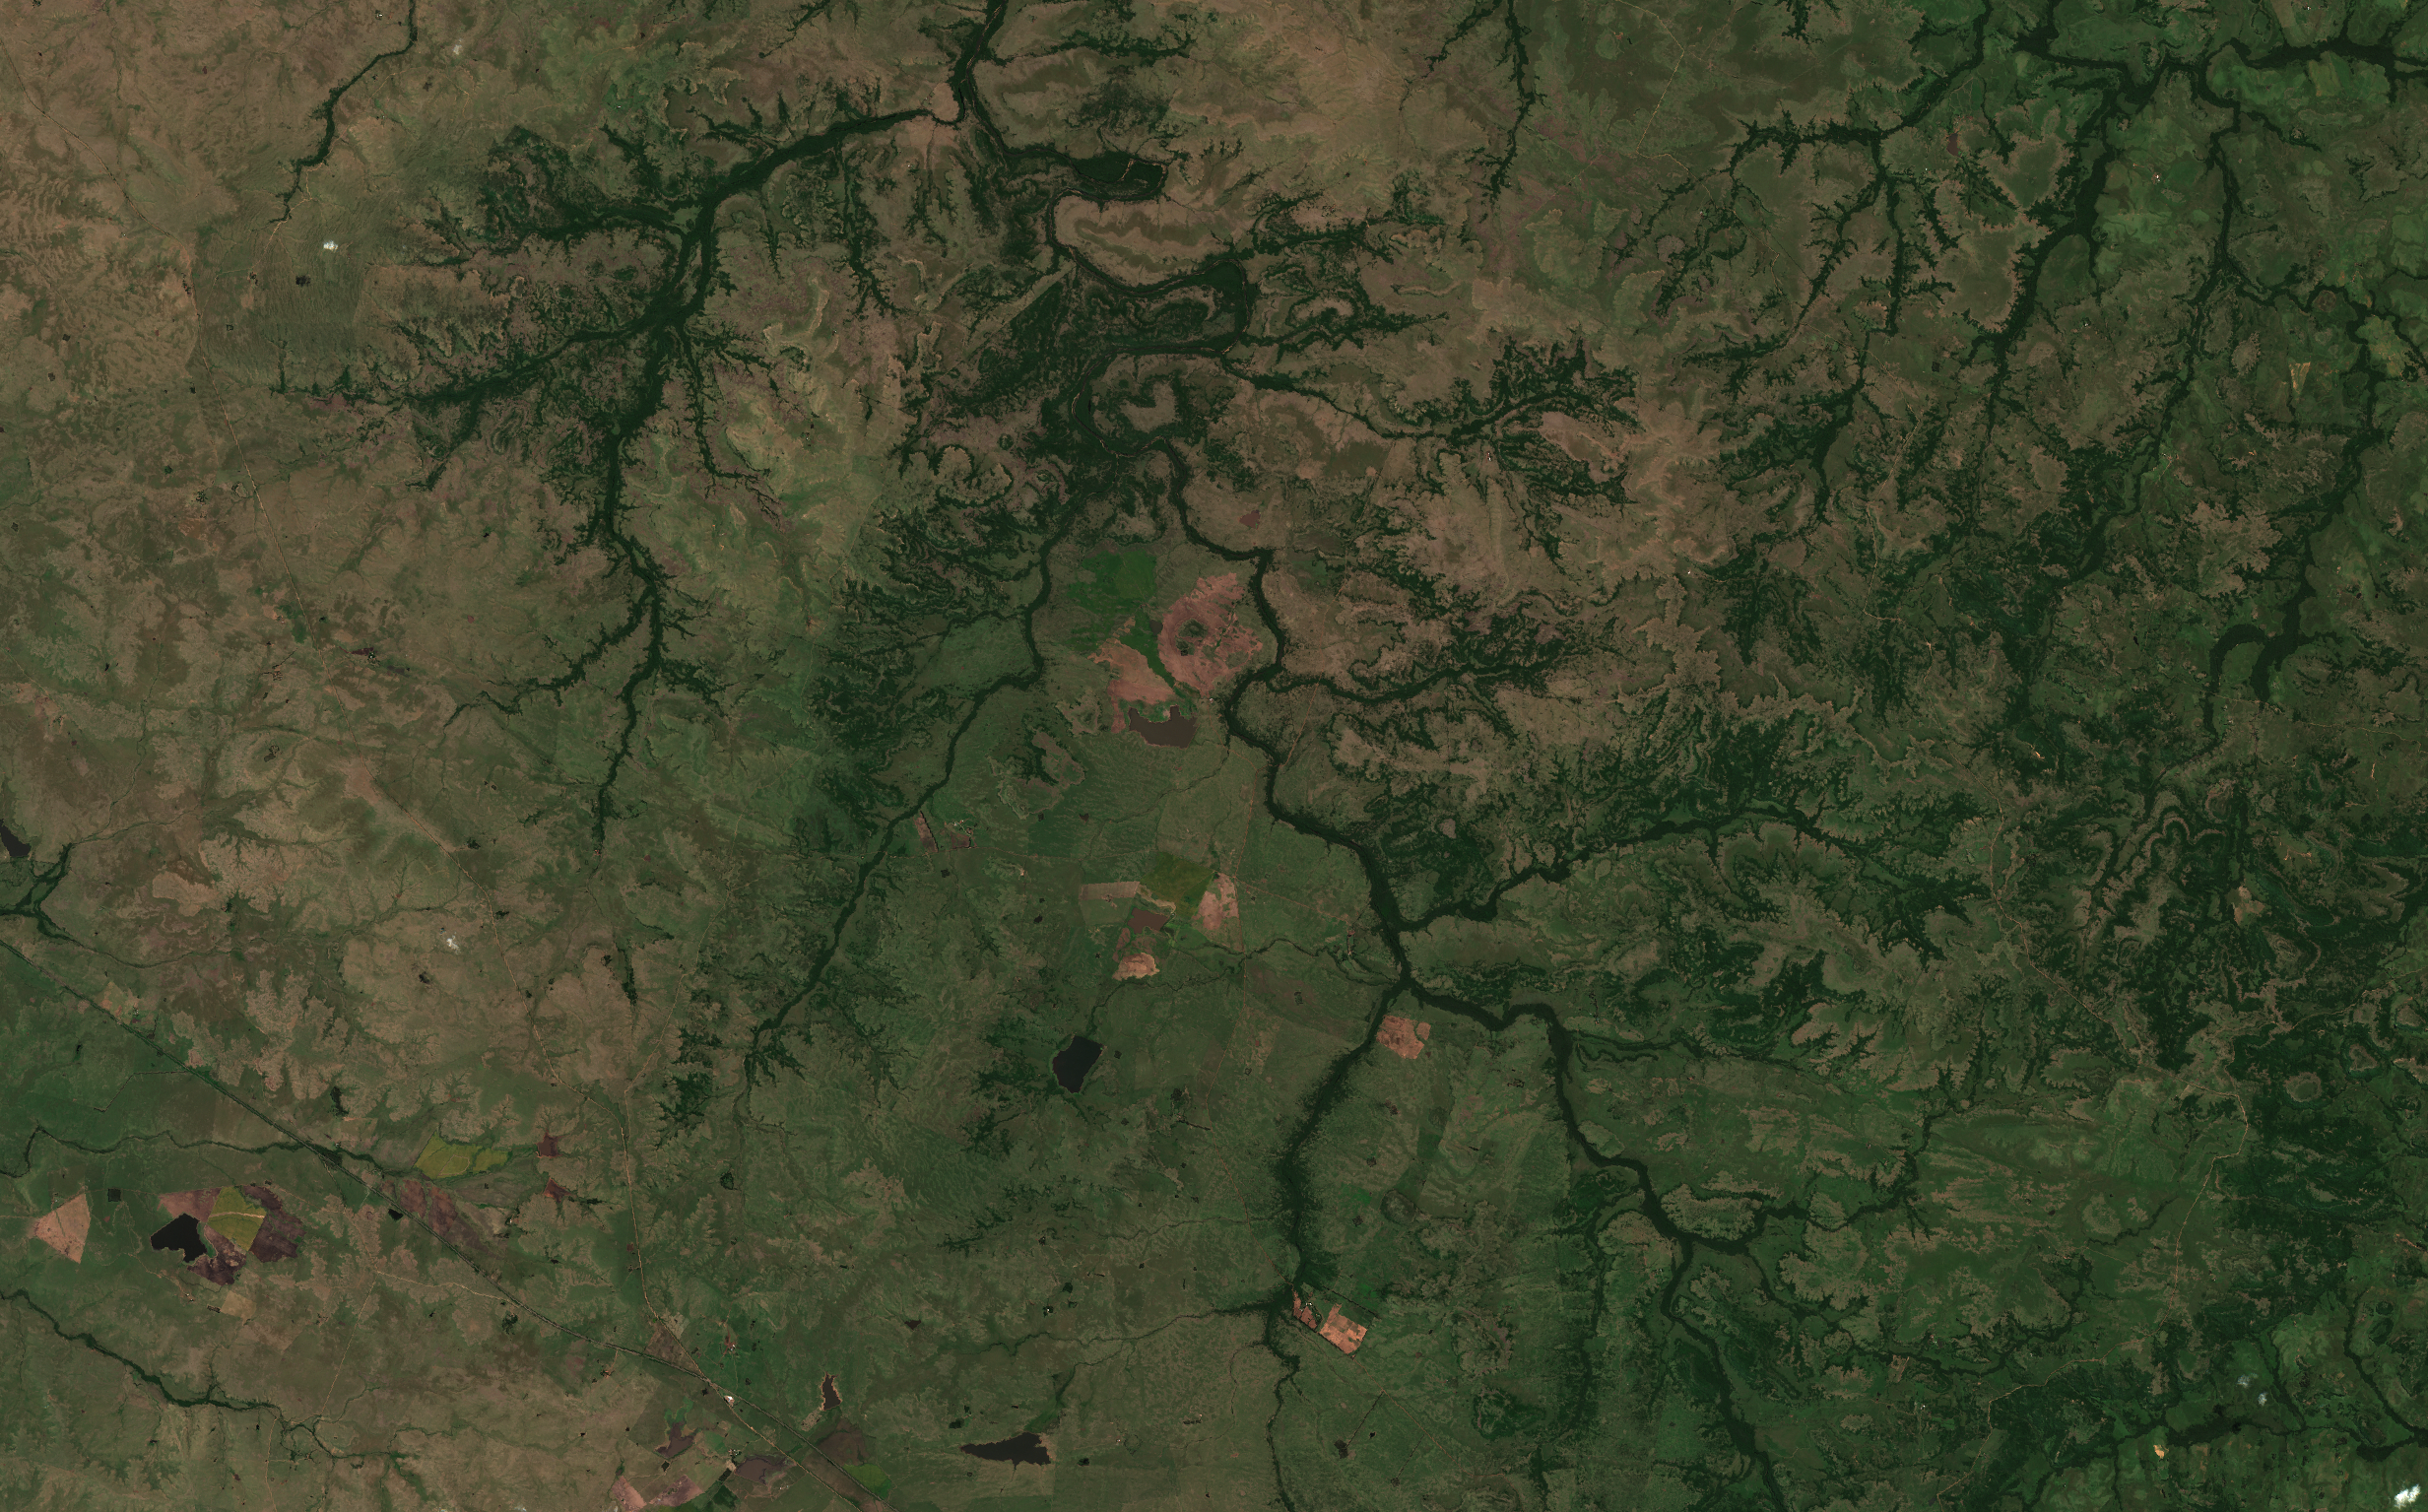
\includegraphics[width=\textwidth,height=4.5cm,keepaspectratio]{img/comparacao/imagem-clean.png}\\[0.2cm]
            {\footnotesize\textbf{Imagem Limpa} --- Alta qualidade}
        \end{center}
        
        \vspace{-0.2cm}
        \begin{center}
            \colorbox{ufal!10}{\parbox{0.9\textwidth}{\centering
                \footnotesize\textbf{Objetivo:} Selecionar automaticamente as melhores imagens para cada período, evitando qualidade intermediária e problemas como nuvens/dados faltantes
            }}
        \end{center}
    \end{column}
    
    \begin{column}{0.48\textwidth}
        \vspace{0.2cm}
        \begin{center}
            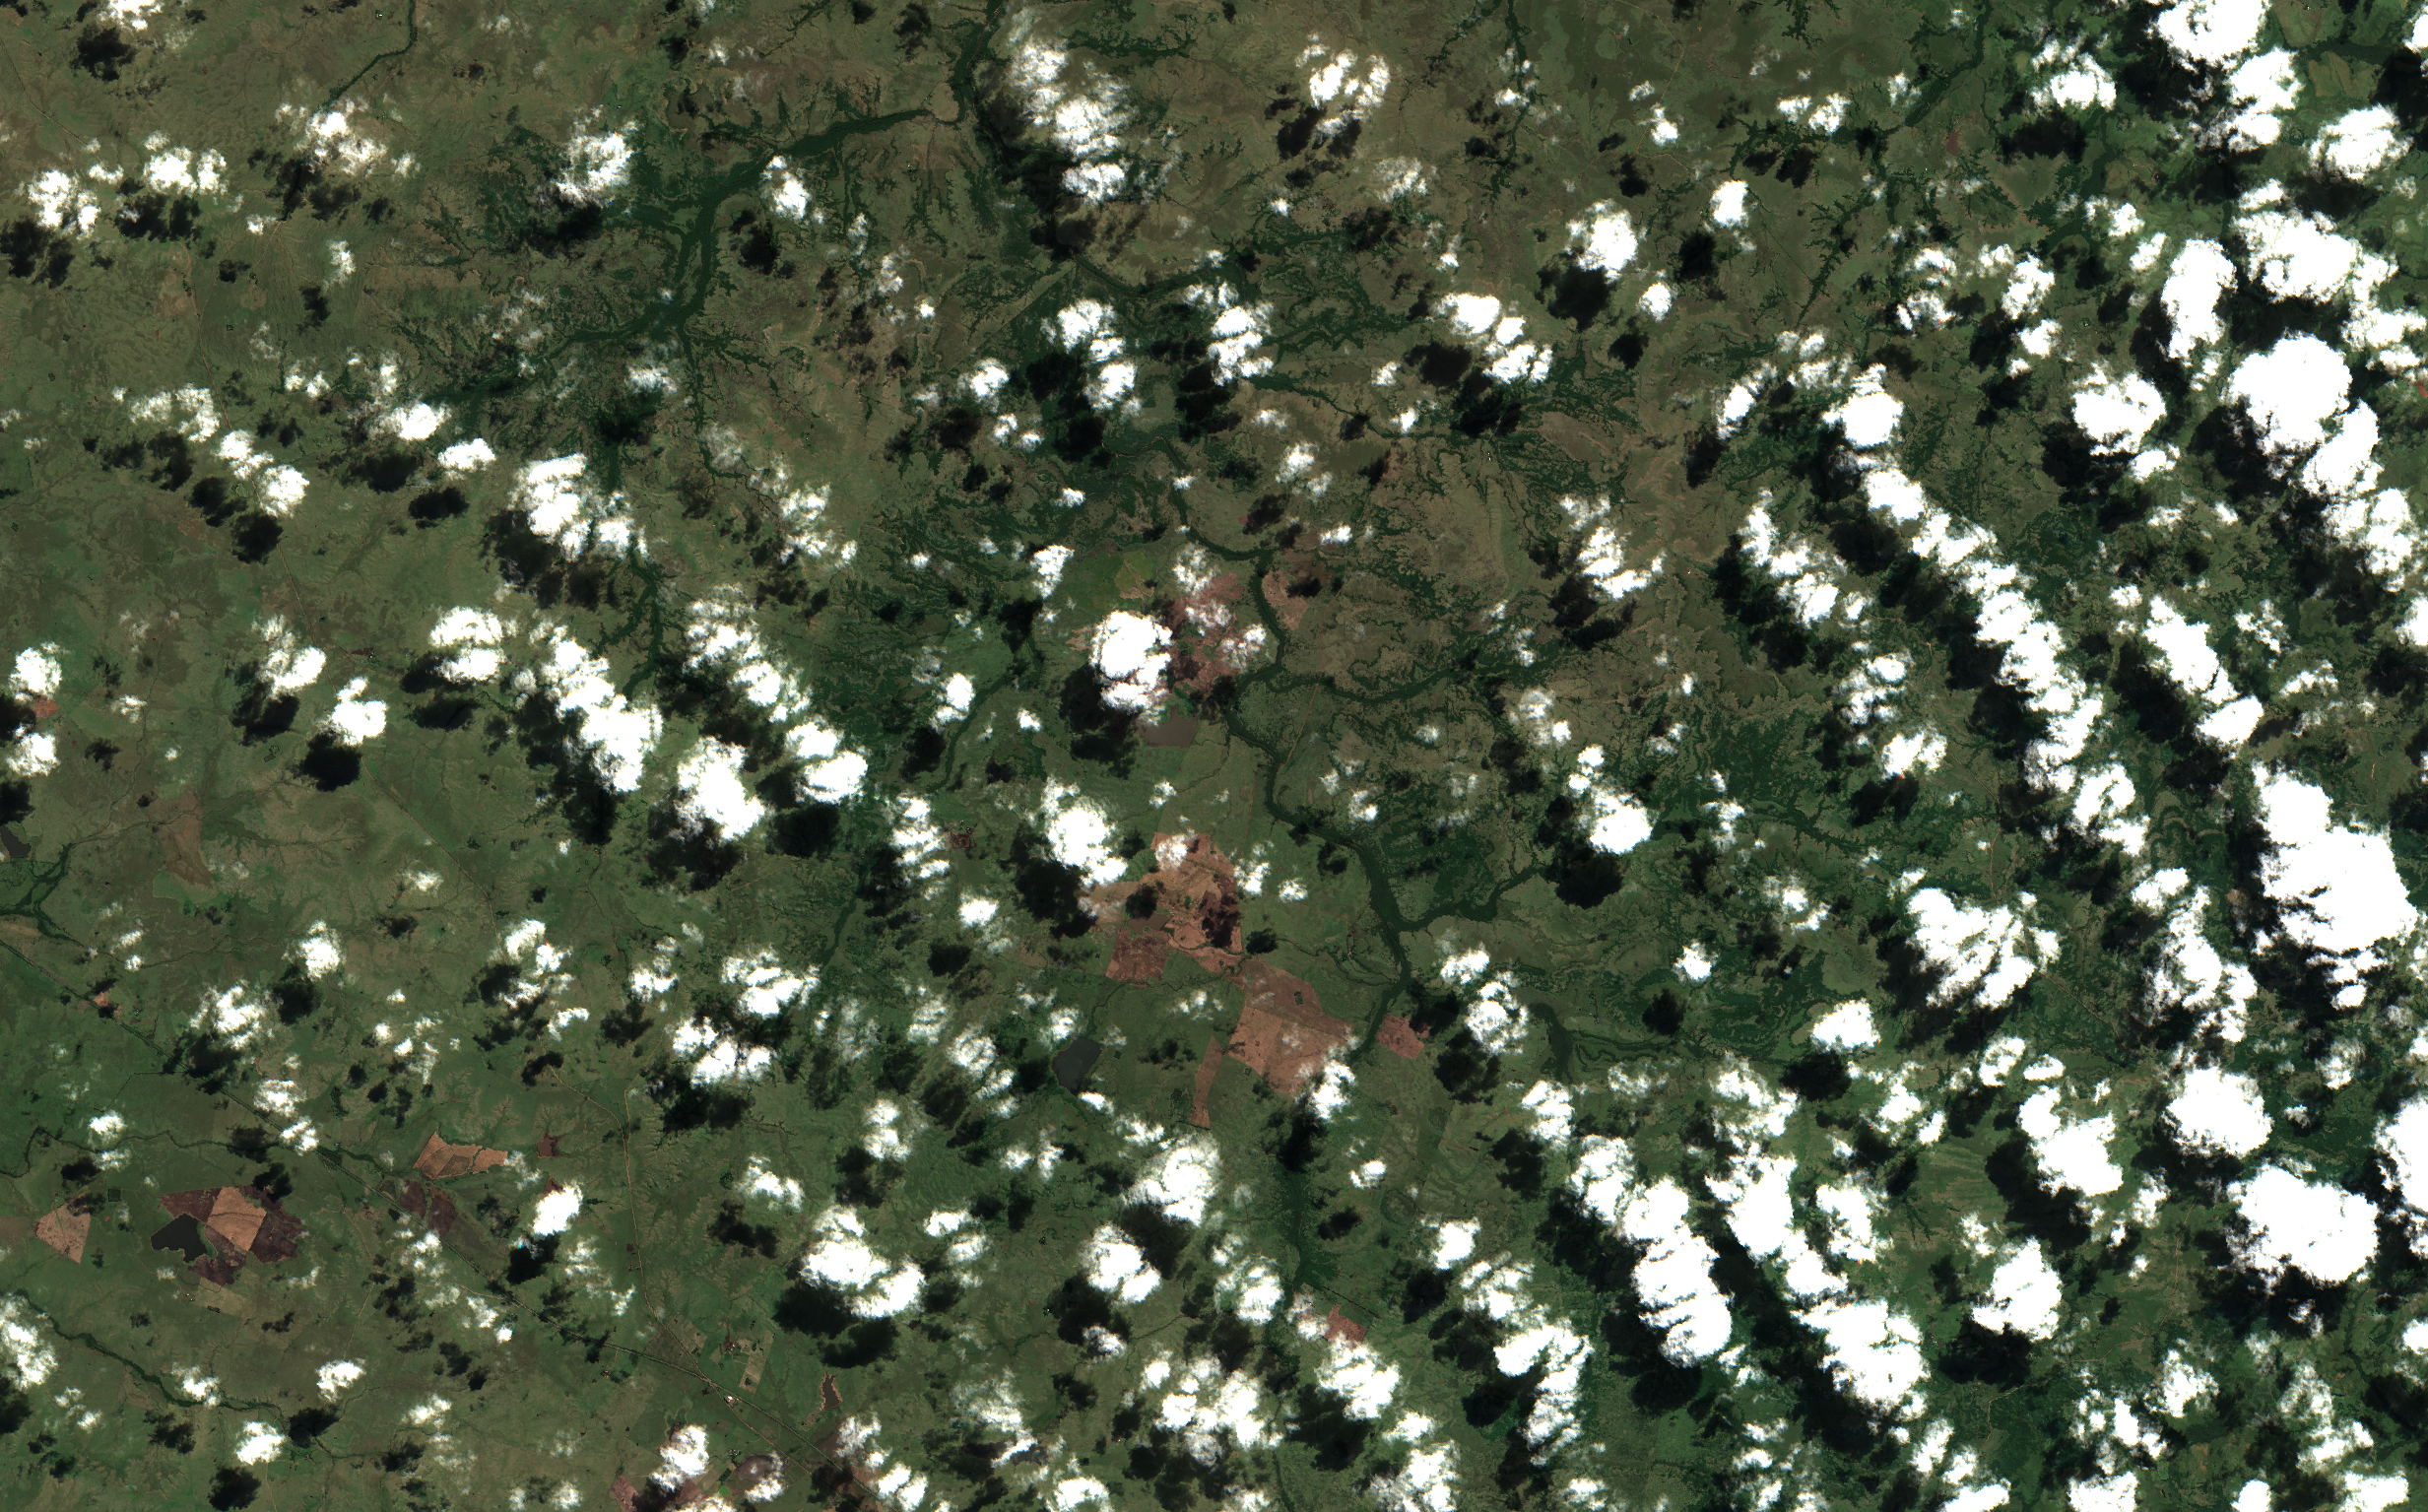
\includegraphics[width=\textwidth,height=3.5cm,keepaspectratio]{img/comparacao/imagem-mid-clean.png}\\[0.2cm]
            
            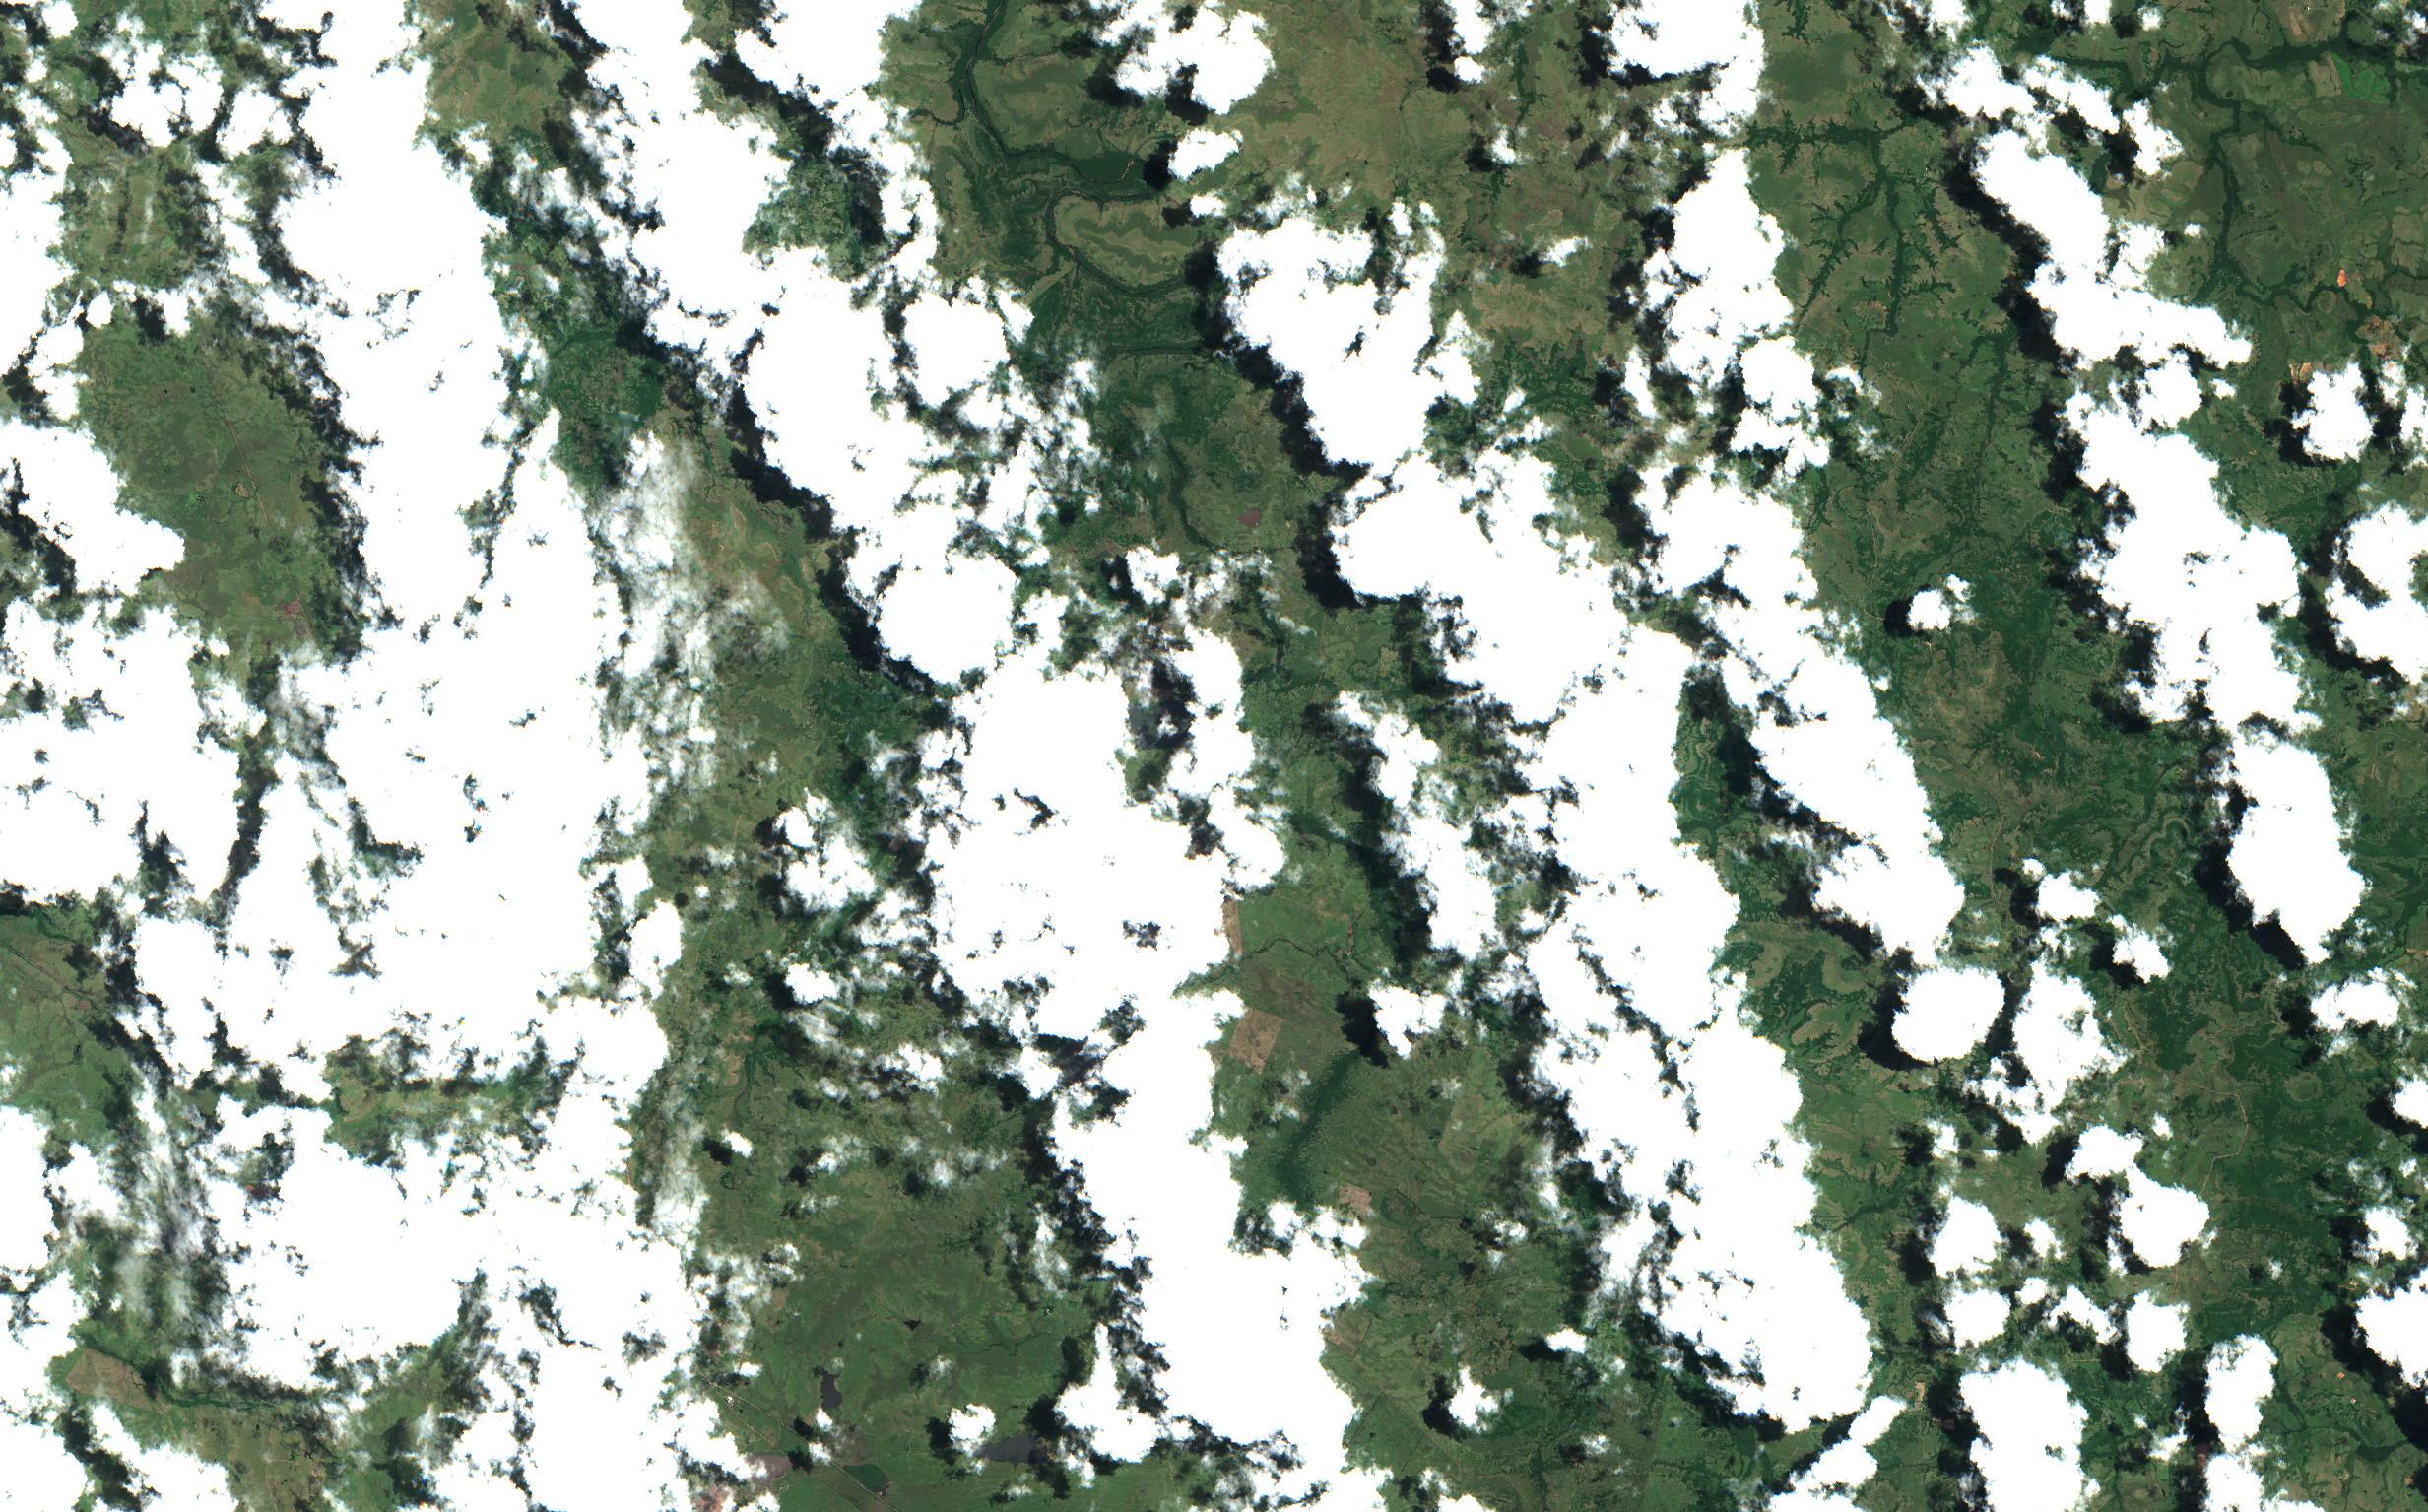
\includegraphics[width=\textwidth,height=3.5cm,keepaspectratio]{img/comparacao/imagem-suja.png}
        \end{center}
    \end{column}
\end{columns}
\end{frame}

% Slide 18: Impacto compacto
\begin{frame}{Impacto e Aplicações}
\vspace{-0.2cm}
\begin{multicols}{2}
    \textbf{\color{ufal}Contribuições:}
    \begin{itemize}
        \item Metodologia híbrida eficiente
        \item Controle de qualidade automático
        \item Continuidade espacial garantida
        \item Aplicável a diferentes UCs
    \end{itemize}
    
    \columnbreak%
    \textbf{\color{success}Aplicações:}
    \begin{itemize}
        \item Monitoramento de desmatamento
        \item Detecção de incêndios
        \item Mudanças de cobertura
        \item Análise multitemporal
    \end{itemize}
\end{multicols}
\end{frame}

% Slide 20: Limitações e Trabalhos Futuros
\begin{frame}{Limitações e Trabalhos Futuros}
\begin{columns}[T]
    \begin{column}{0.48\textwidth}
        \textbf{\color{accent}Limitações:}
        \begin{itemize}
            \item Espaçamento variável entre mosaicos devido ao clima
            \item Cobertura subótima em regiões com alta nebulosidade
            \item Dependência de sensoriamento óptico
        \end{itemize}
    \end{column}
    \begin{column}{0.48\textwidth}
        \textbf{\color{ufal}Próximos Passos:}
        \begin{itemize}
            \item \textbf{Integração SAR} para áreas nubladas
            \item \textbf{Janelas temporais maiores} para cobrir lacunas
            \item \textbf{Fusão de imagens} com base em máscaras de nuvens
            \item \textbf{Expansão} para diferentes perfis climáticos
        \end{itemize}
    \end{column}
\end{columns}

\vspace{0.3cm}
\begin{center}
    \colorbox{success!10}{\parbox{10cm}{\centering
        \textbf{Futuro:} Completar mosaicos parcialmente nublados com recortes limpos de outras imagens usando comparação de máscaras de nuvens
    }}
\end{center}
\end{frame}

% Slide 21: Final
\begin{frame}[plain]
    \begin{center}
        {\Large\textbf{Agradecimentos}}\\[0.5cm]

        Agradecimentos aos meus orientadores, à Universidade Federal de Alagoas,\\
        ao Instituto de Computação e à organização do SBPO 2025\@.\\[0.7cm]

        Obrigado a todos presentes!

        \includegraphics[height=1.5cm]{img/ufal.jpg}\hspace{0.5cm}%
        \includegraphics[height=1.5cm]{img/logo-ic.png}\hspace{0.5cm}%
        \includegraphics[height=1.5cm]{img/sbpo2025-header-logo.png}\\[0.7cm]
        
        {\Huge\textbf{Perguntas?}}
    \end{center}
\end{frame}

\end{document}